%!TEX root = Nanomat.tex
\ctitle{Kolloider}

\paragraph{Kolloid} En \idx{kolloid} er en ikke-homogen løsning av to eller flere komponenter der den ene komponenten finnes i form av dråper med en størrelse mellom \SI{1}{\nano\meter} og \SI{1000}{\nano\meter} som er jevnt fordelt i løsningen. Melk består i hovedsak av dråper med smørfett i vannløsning\footnote{Mmm.}, og er dermed en kolloid.

\cstitle{Surfaktanter}
Surfaktanter er molekyler med et hydrofilt (polart) ``hode'' og en hydrofob (upolar) ``hale''. Hvis disse tilsettes et system av to uløselige media, vil slike surfaktanter spontant posisjonere seg i grenseflaten mellom de to mediene slik at den hydrofile enden befinner seg i det polare mediet og den hydrofobe enden befinner seg i det upolare mediet. Olje og vann kommer til å bli brukt i stedet for ``polar løsning'' og ``upolar løsning'' i dette kapittelet, men det kan som regel generaliseres. Dette kan danne forskjellige strukturer, avhengig av \emph{formen på surfaktantmolekylet}. 

\paragraph{Miceller} Hvis surfaktanten består av et bredt polart hode og en smal upolar hale, så vil det i grenseflaten mellom to medier dannes en \emph{miceller}\index{micelle} der de upolare endene går mot sentrum og de polare hodene stikker ut. Som Figur~\ref{fig:micelle} viser, kan disse transportere dråper med olje rundt omkring i en vannløsning. Hvis surfaktantkonsentrasjonen er liten vil micellene være kulerunde, med en diameter som er bestemt av lengden på hydrokarbonkjeden og det polare hodet. Miceller er dynamiske systemer der individuelle surfaktantmolekyler stadig byttes ut (alle molekylene i en gitt micelle vil være byttet ut i løpet av noen mikrosekunder).
\begin{figure}[H]
	\bmd\centering
	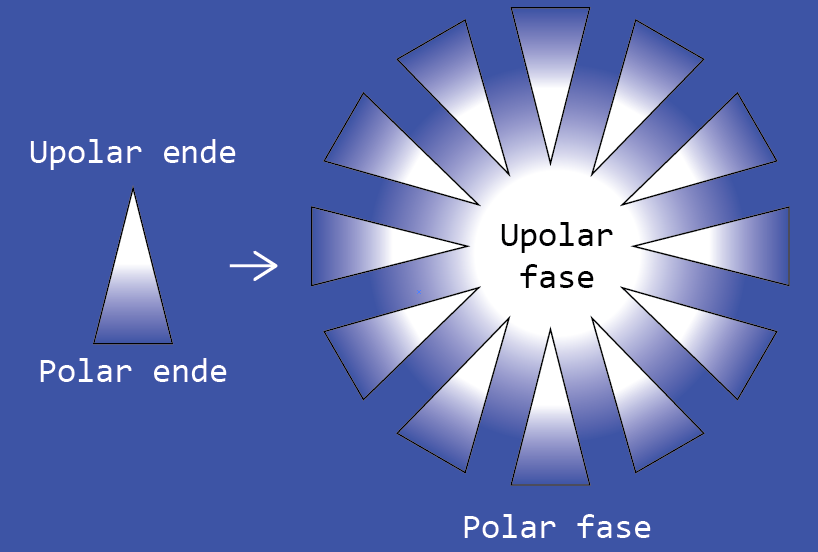
\includegraphics[width=0.8\linewidth]{micelle.png}
	\caption{Skjematisk illustrasjon av en surfaktant med et bredt polart hode og en smal upolar hale (typisk en ikke-forgrenet karbonkjede) som gir opphav til en micelle, som kan transportere dråper av olje i vannløsning.}
	\label{fig:micelle}
\emd\end{figure}

\paragraph{Reverserte miceller} Hvis surfaktanten består av et smalt polart hode og en bred upolar hale, så vil det dannes \emph{reverserte miceller}\index{reversert micelle} på samme måte som med miceller. Disse vil kunne transportere vann rundt omkring i en oljeløsning, som vist i Figur~\ref{fig:reversemicelle}. En egenskap ved reverserte miceller som man ikke observerer i miceller, er at reverserte miceller kan kollapse til én stor micelle, utveksle innhold, og så dele seg til to reverserte miceller igjen. En andre egenskap som er unik for reverserte miceller, er at størrelsen deres øker lineært med andelen vann i systemet; diameteren øker fra \SI{4}{\nano\meter} til \SI{18}{\nano\meter} når vannmengden $w=[\ce{H2O}]/[\ce{surfaktant}]$ øker fra $2$ til $20$.
\begin{figure}[H]
	\bmd\centering
	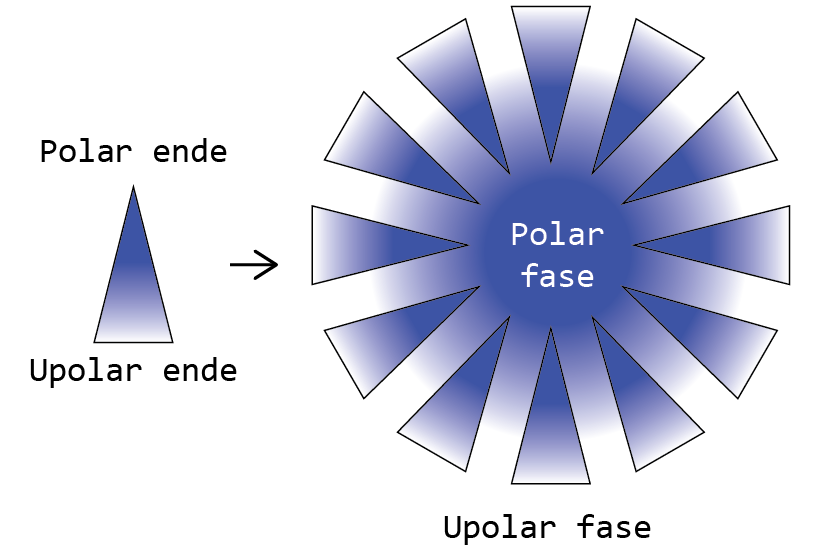
\includegraphics[width=0.8\linewidth]{reversemicelle.png}
	\caption{Skjematisk illustrasjon av en surfaktant med et smalt polart hode og en bred upolar hale (typisk en forgrenet karbonkjede) som gir opphav til en reversert micelle, som kan transportere dråper av et polart stoff i et upolart miljø.}
	\label{fig:reversemicelle}
\emd\end{figure}

\paragraph{Andre strukturer}
\begin{itemize}
	\item Dersom man har riktig mye vann i en oljerik løsning med surfaktanter, vil man i stedet observere at surfaktantene danner kanaler slik at man har alternerende regioner med olje og vann.
	\item Enda mer vann vil føre til at surfaktantene danner plane filmer (såkalt lamellær fase) som gjør systemet \idx{birefringent}, det vil si at det bryter lys forskjellig i forskjellige retninger.
	\item En siste mulig konfigurasjon av surfaktantene er såkalte \idx{superaggregat}er der surfaktantfilmen krummer seg innover og danner lag på lag med kulerunde strukturer (og sammenkoblede kanaler både på innsiden og utsiden av superaggregatet). Alle disse forskjellige strukturene kan (visstnok) forklares ut i fra geometrien til surfaktantmolekylene.
\end{itemize}

\paragraph{Reverserte miceller som nanoreaktorer} Egenskapen reverserte miceller har til å utveksle innhold kan brukes til å lage nanostrukturerte materialer med en helt bestemt størrelse på partiklene. Prosessen, slik den er beskrevet i Figur 18.9 i Bréchnigac et. al., gjengis her på norsk:
\begin{enumerate}
	\item Vi begynner med to separate løsninger med reverserte miceller. I den ene løsningen inneholder de reverserte micellene reaktant \ce{A}, i den andre inneholder de reaktant \ce{B}.
	\item Løsningene blandes. De reverserte micellene utveksler materiale.
	\item \ce{A} og \ce{B} reagerer inni cellene og danner produktet \ce{AB}. Reaksjonen er begrenset av størrelsen på micellene, så produktet vil være i form av nanopartikler og kan dermed ha forskjellige egenskaper fra bulk-materialet. Siden størrelsen på de reverserte micellene avhenger av vanninholdet, kan nanopartiklenes størrelse justeres ved å justere vanninnholdet.
	\item Micellene med produkt ekstraheres fra løsningen.
\end{enumerate}
Hvis vi bare hadde reagert \ce{A} og \ce{B} uten denne prosessen, ville vi fått produktet i form av bulkmaterialet. 
